% ********** Rozdział 4 **********
\chapter{Prezentacja warstwy użytkowej projektu}
\section{Zrzuty ekranu aplikacji i ich opisy}

Poniżej znajduje się zestaw zrzutów ekranu przedstawiających różne funkcje i operacje w Panelu Kontrolnym Dostawców. W panelu wyróżniono następujące sekcje:
\begin{itemize}
    \item Pierwszy textbox i zielony przycisk: \textbf{Załaduj listę dostawców}.
    \item Drugi textbox i niebieski przycisk: \textbf{Dodaj nowego dostawcę}.
    \item Trzeci textbox i niebieski przycisk: \textbf{Aktualizuj dane istniejącego dostawcy}.
    \item Czwarty textbox i czerwony przycisk: \textbf{Usuń dostawcę według ID}.
\end{itemize}

\subsection{Funkcjonalności panelu}
W aplikacji główny widok umożliwia wykonywanie podstawowych operacji CRUD (Create, Read, Update, Delete) na danych dostawców. Na przykład, na rysunku \ref{fig:suppliers_test_1} widzimy ekran startowy panelu, gdzie możemy załadować listę dostawców przy użyciu zielonego przycisku. Po wczytaniu danych, jak na rysunku \ref{fig:suppliers_test_2}, użytkownik może przystąpić do dodawania, modyfikacji lub usuwania danych.

Na rysunku \ref{fig:suppliers_test_3} zaprezentowano przykład dodawania nowego dostawcy, gdzie w drugim textboxie należy wprowadzić szczegóły, a następnie kliknąć \textbf{Dodaj}. System wyświetla potwierdzenie sukcesu operacji, jak pokazano na rysunku \ref{fig:suppliers_test_4}.

Z kolei na rysunku \ref{fig:suppliers_test_6} pokazano możliwość aktualizacji danych istniejącego dostawcy, za pomocą trzeciego textboxa i przycisku \textbf{Aktualizuj}. Po dokonaniu zmian lista dostawców zostaje odświeżona, co widać na rysunku \ref{fig:suppliers_test_7}. Dodatkowo użytkownik może usuwać dostawców, podając ich ID w czwartym textboxie i klikając czerwony przycisk, jak pokazano na rysunku \ref{fig:suppliers_test_8}.

W przypadku błędów, takich jak nieprawidłowe dane wejściowe, aplikacja wyświetla odpowiednie komunikaty, co przedstawiono na rysunku \ref{fig:suppliers_test_9_1}.

\subsection{Rozszerzenia aplikacji}
Poza obsługą dostawców aplikacja zawiera panele umożliwiające zarządzanie produktami i kategoriami. Jak widać na rysunku \ref{fig:suppliers_test_10}, panel produktów działa na podobnych zasadach, umożliwiając dodawanie, modyfikację i usuwanie danych produktów. Panel kategorii, przedstawiony na rysunku \ref{fig:suppliers_test_11}, pozwala na podobne operacje w kontekście zarządzania kategoriami.

\subsection{Dokumentacja API}
Rysunek \ref{fig:swagger} przedstawia dokumentację API wygenerowaną za pomocą narzędzia Swagger. Dzięki tej dokumentacji możliwe jest łatwe zrozumienie struktury zapytań i odpowiedzi w aplikacji. API zostało zaprojektowane w sposób uniwersalny, umożliwiając interakcję z backendem nie tylko za pomocą aplikacji napisanej w Windows Forms, ale również przy użyciu dowolnej platformy czy frameworka, takich jak:
\begin{itemize}
    \item aplikacje webowe oparte na frameworkach takich jak \textbf{React}, \textbf{Angular} czy \textbf{Vue.js},
    \item aplikacje mobilne tworzone w \textbf{Flutter}, \textbf{React Native} lub \textbf{Swift},
    \item aplikacje desktopowe budowane z użyciem innych frameworków.
\end{itemize}

Dzięki temu podejściu frontend może być dostosowany do różnych potrzeb użytkowników, co znacząco zwiększa wszechstronność i skalowalność rozwiązania. Przykładowo, firma może zaimplementować aplikację mobilną do szybkiego zarządzania dostawcami, podczas gdy inny zespół pracuje nad rozbudowaną aplikacją webową dla większych operacji.

\subsection{Zrzuty ekranu}

\begin{figure}[h!]
    \centering
    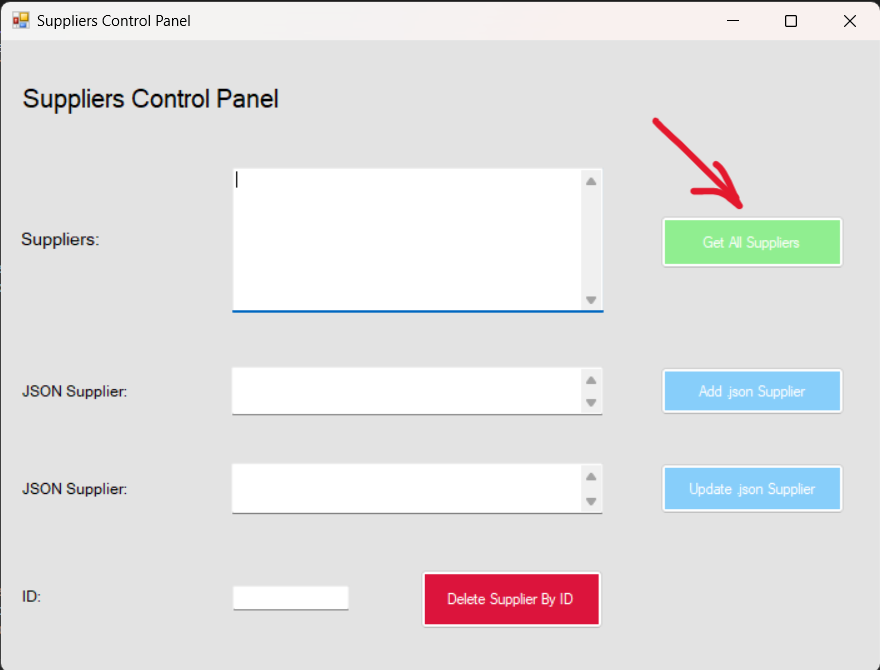
\includegraphics[width=0.8\textwidth]{img_tests/suppliers_test_1.png}
    \caption{Ekran startowy panelu. Funkcja załaduj listę dostawców za pomocą zielonego przycisku.}
    \label{fig:suppliers_test_1}
\end{figure}

\begin{figure}[h!]
    \centering
    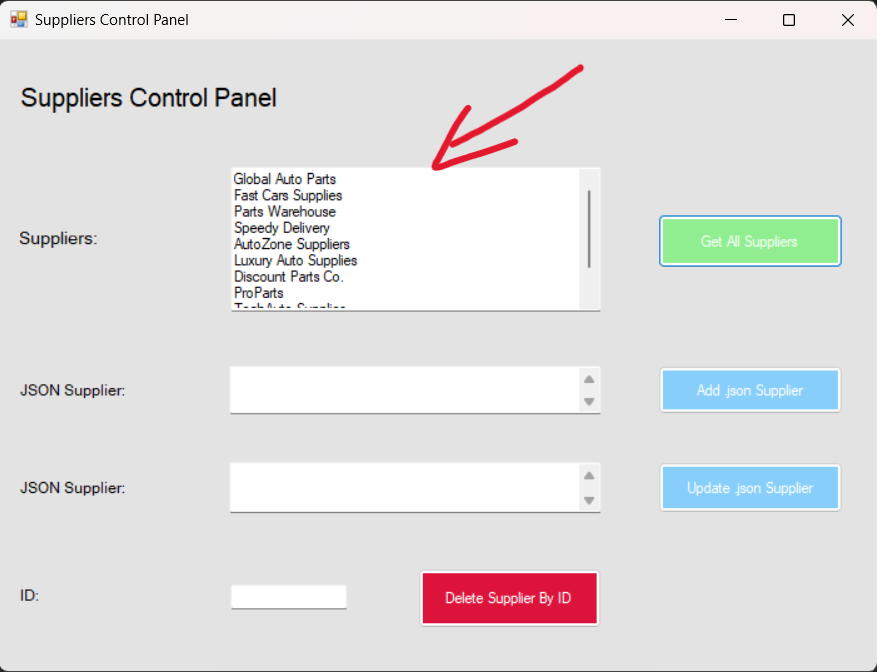
\includegraphics[width=0.8\textwidth]{img_tests/suppliers_test_2.png}
    \caption{Lista dostawców załadowana w pierwszym polu tekstowym po kliknięciu przycisku \textbf{Załaduj}.}
    \label{fig:suppliers_test_2}
\end{figure}

\begin{figure}[h!]
    \centering
    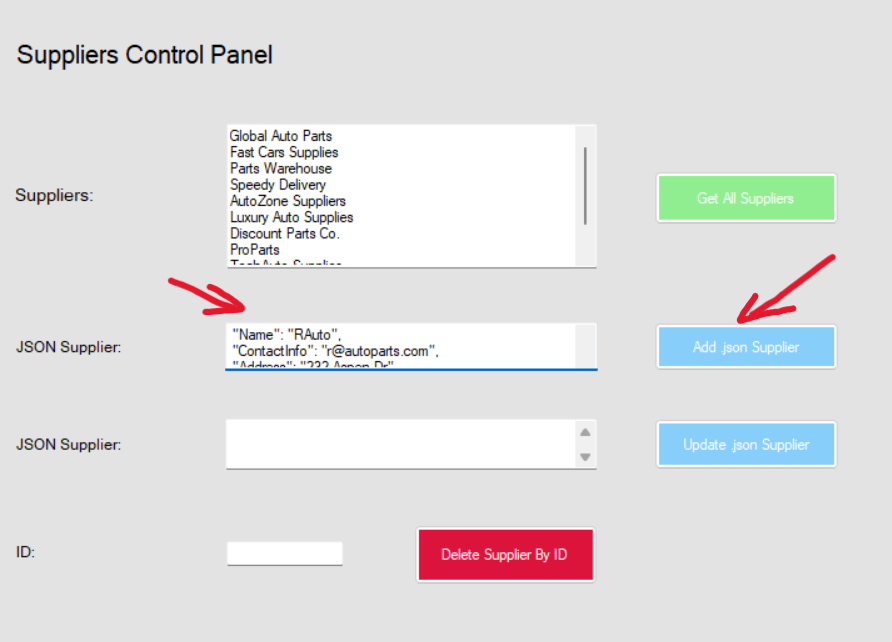
\includegraphics[width=0.8\textwidth]{img_tests/suppliers_test_3.png}
    \caption{Dodawanie nowego dostawcy. Drugi tekstboks służy do wprowadzania danych nowego dostawcy. Kliknij \textbf{Dodaj}, aby zatwierdzić.}
    \label{fig:suppliers_test_3}
\end{figure}

\begin{figure}[h!]
    \centering
    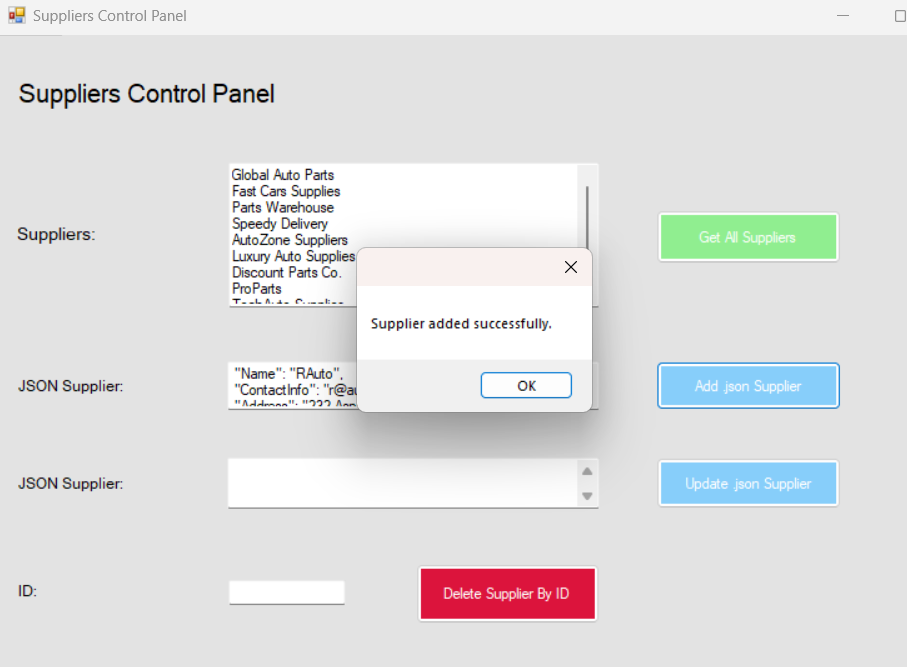
\includegraphics[width=0.8\textwidth]{img_tests/suppliers_test_4.png}
    \caption{Potwierdzenie pomyślnego dodania nowego dostawcy.}
    \label{fig:suppliers_test_4}
\end{figure}

\begin{figure}[h!]
    \centering
    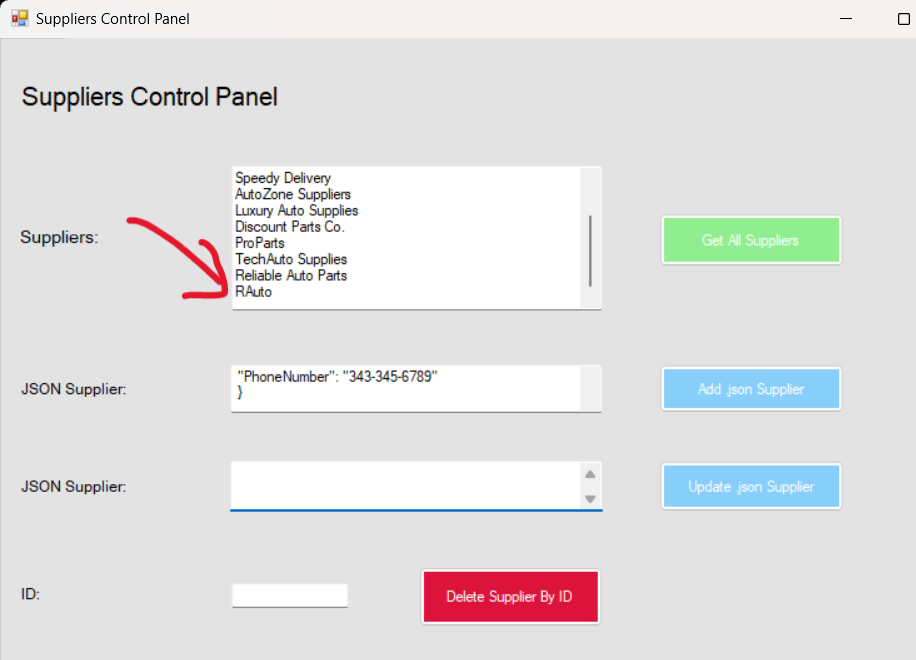
\includegraphics[width=0.8\textwidth]{img_tests/suppliers_test_5.png}
    \caption{Potwierdzenie pomyślnego dodania nowego dostawcy.}
    \label{fig:suppliers_test_5}
\end{figure}

\begin{figure}[h!]
    \centering
    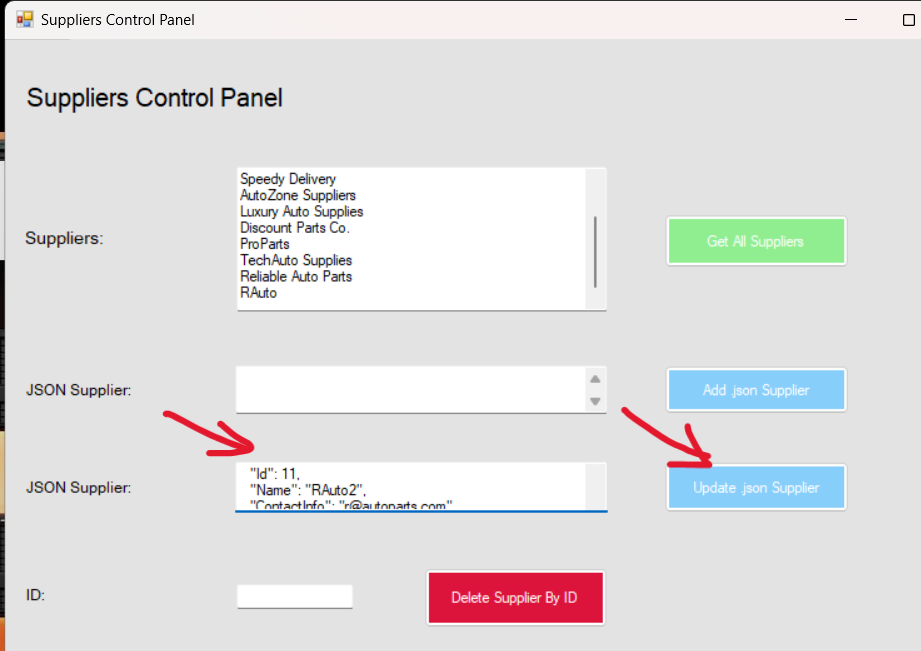
\includegraphics[width=0.8\textwidth]{img_tests/suppliers_test_6.png}
    \caption{Wprowadzanie danych dostawcy do aktualizacji w trzecim tekście i zatwierdzanie przyciskiem \textbf{Aktualizuj}.}
    \label{fig:suppliers_test_6}
\end{figure}

\begin{figure}[h!]
    \centering
    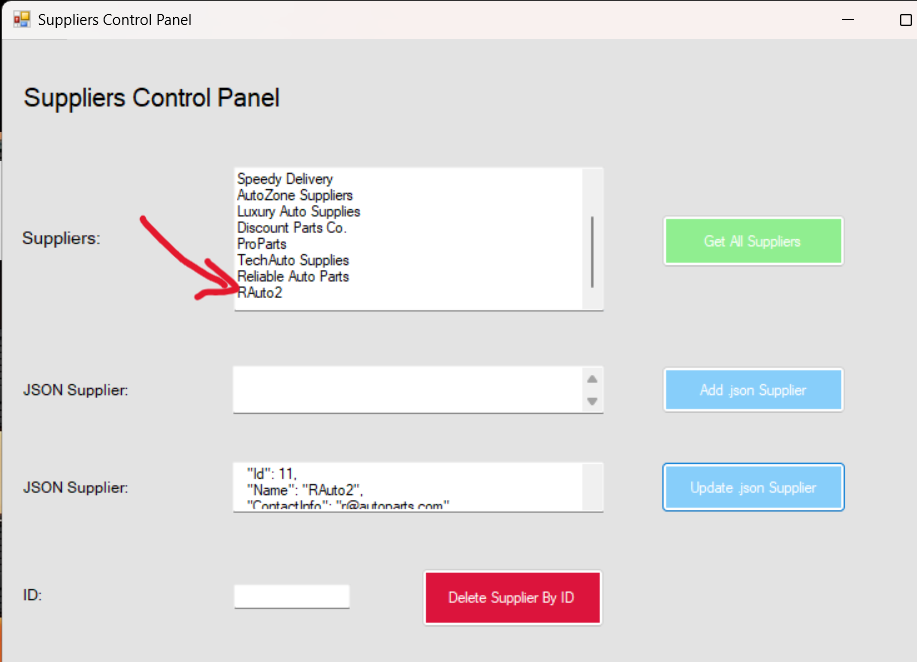
\includegraphics[width=0.8\textwidth]{img_tests/suppliers_test_7.png}
    \caption{Lista dostawców wczytana po modyfikacji z możliwością usunięcia rekordu po ID.}
    \label{fig:suppliers_test_7}
\end{figure}

\begin{figure}[h!]
    \centering
    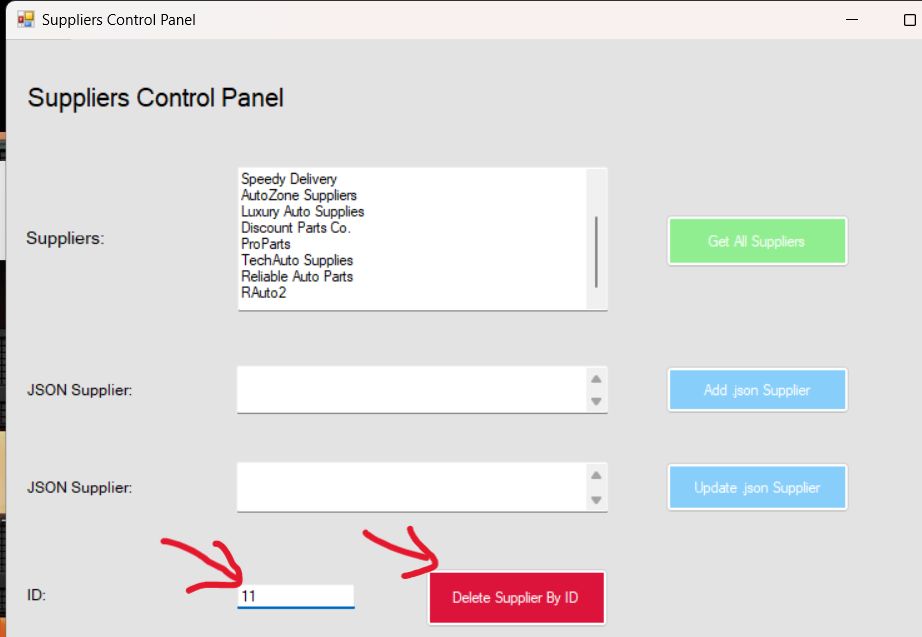
\includegraphics[width=0.8\textwidth]{img_tests/suppliers_test_8.png}
    \caption{Usunięcie dostawcy po ID za pomocą czwartego tekstowego pola i czerwonego przycisku \textbf{Usuń}.}
    \label{fig:suppliers_test_8}
\end{figure}

\begin{figure}[h!]
    \centering
    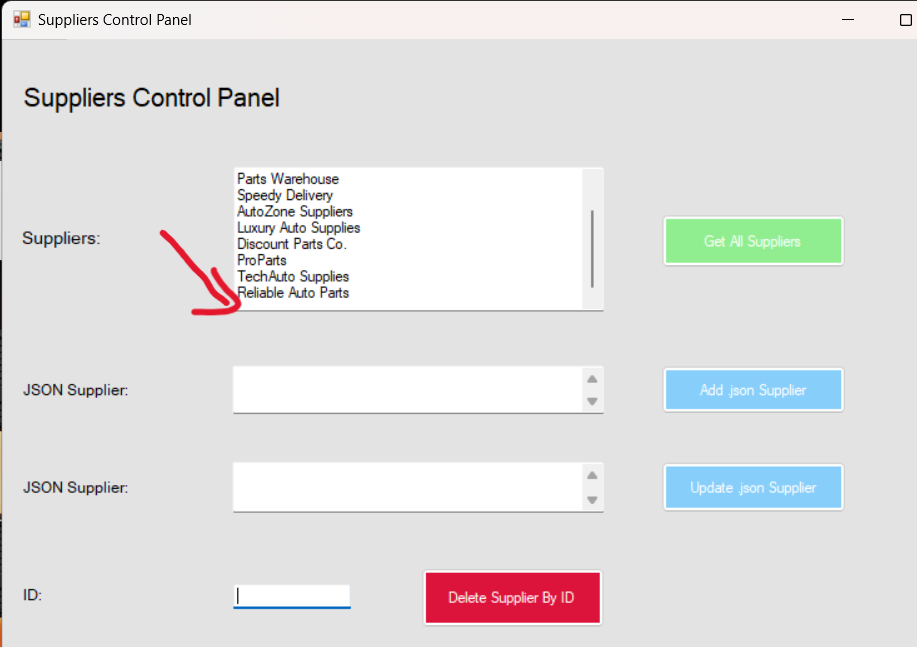
\includegraphics[width=0.8\textwidth]{img_tests/suppliers_test_9.png}
    \caption{Wyświetlenie danych po usunięciu.}
    \label{fig:suppliers_test_9}
\end{figure}

\begin{figure}[h!]
    \centering
    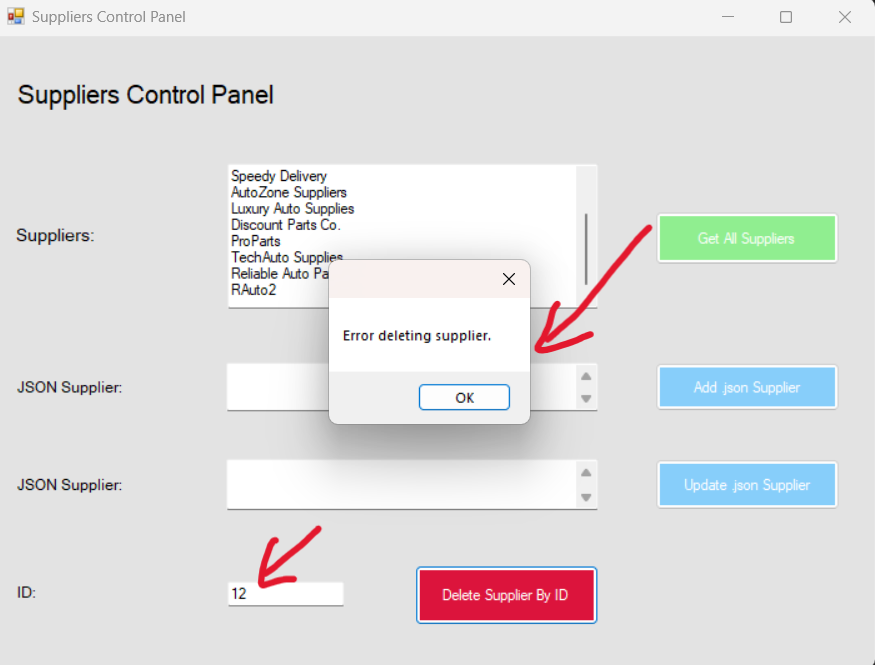
\includegraphics[width=0.8\textwidth]{img_tests/suppliers_test_9_1.png}
    \caption{Wyświetlenie błędu lub informacji o nieprawidłowych danych wprowadzonego dostawcy.}
    \label{fig:suppliers_test_9_1}
\end{figure}


\begin{figure}[h!]
    \centering
    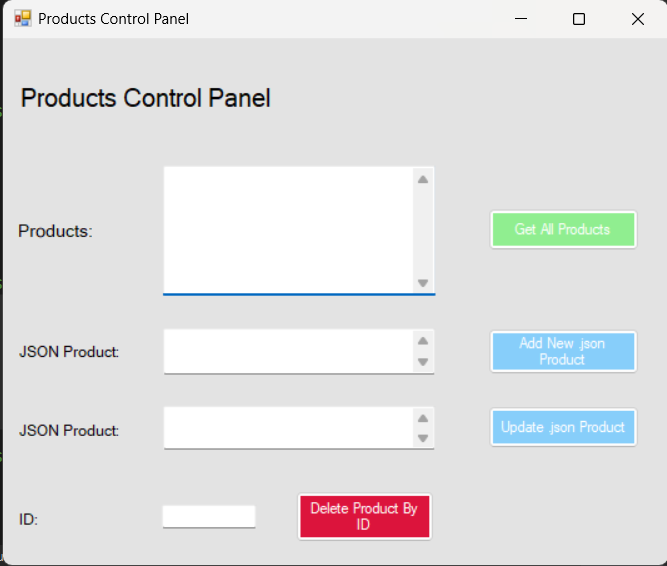
\includegraphics[width=0.8\textwidth]{img_tests/suppliers_test_10.png}
    \caption{Panel zarządzania produktami z funkcjami podobnymi do Panelu Dostawców.}
    \label{fig:suppliers_test_10}
\end{figure}

\begin{figure}[h!]
    \centering
    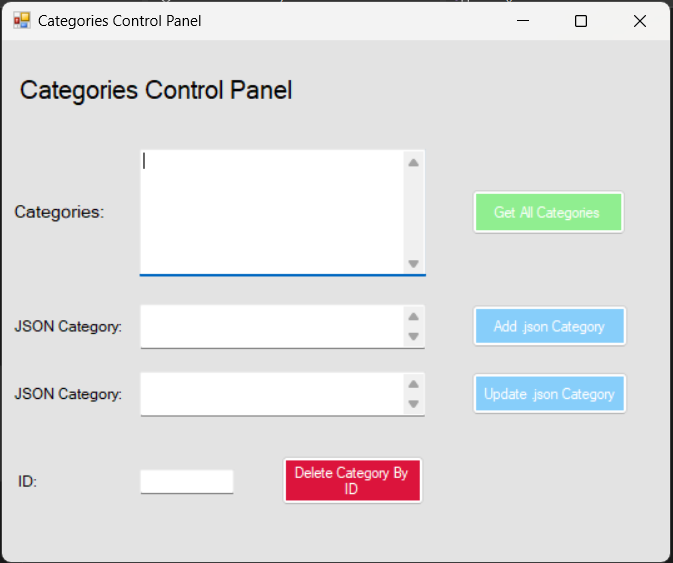
\includegraphics[width=0.8\textwidth]{img_tests/suppliers_test_11.png}
    \caption{Panel zarządzania kategoriami z możliwością dodawania, aktualizowania i usuwania kategorii.}
    \label{fig:suppliers_test_11}
\end{figure}

\begin{figure}[h!]
    \centering
    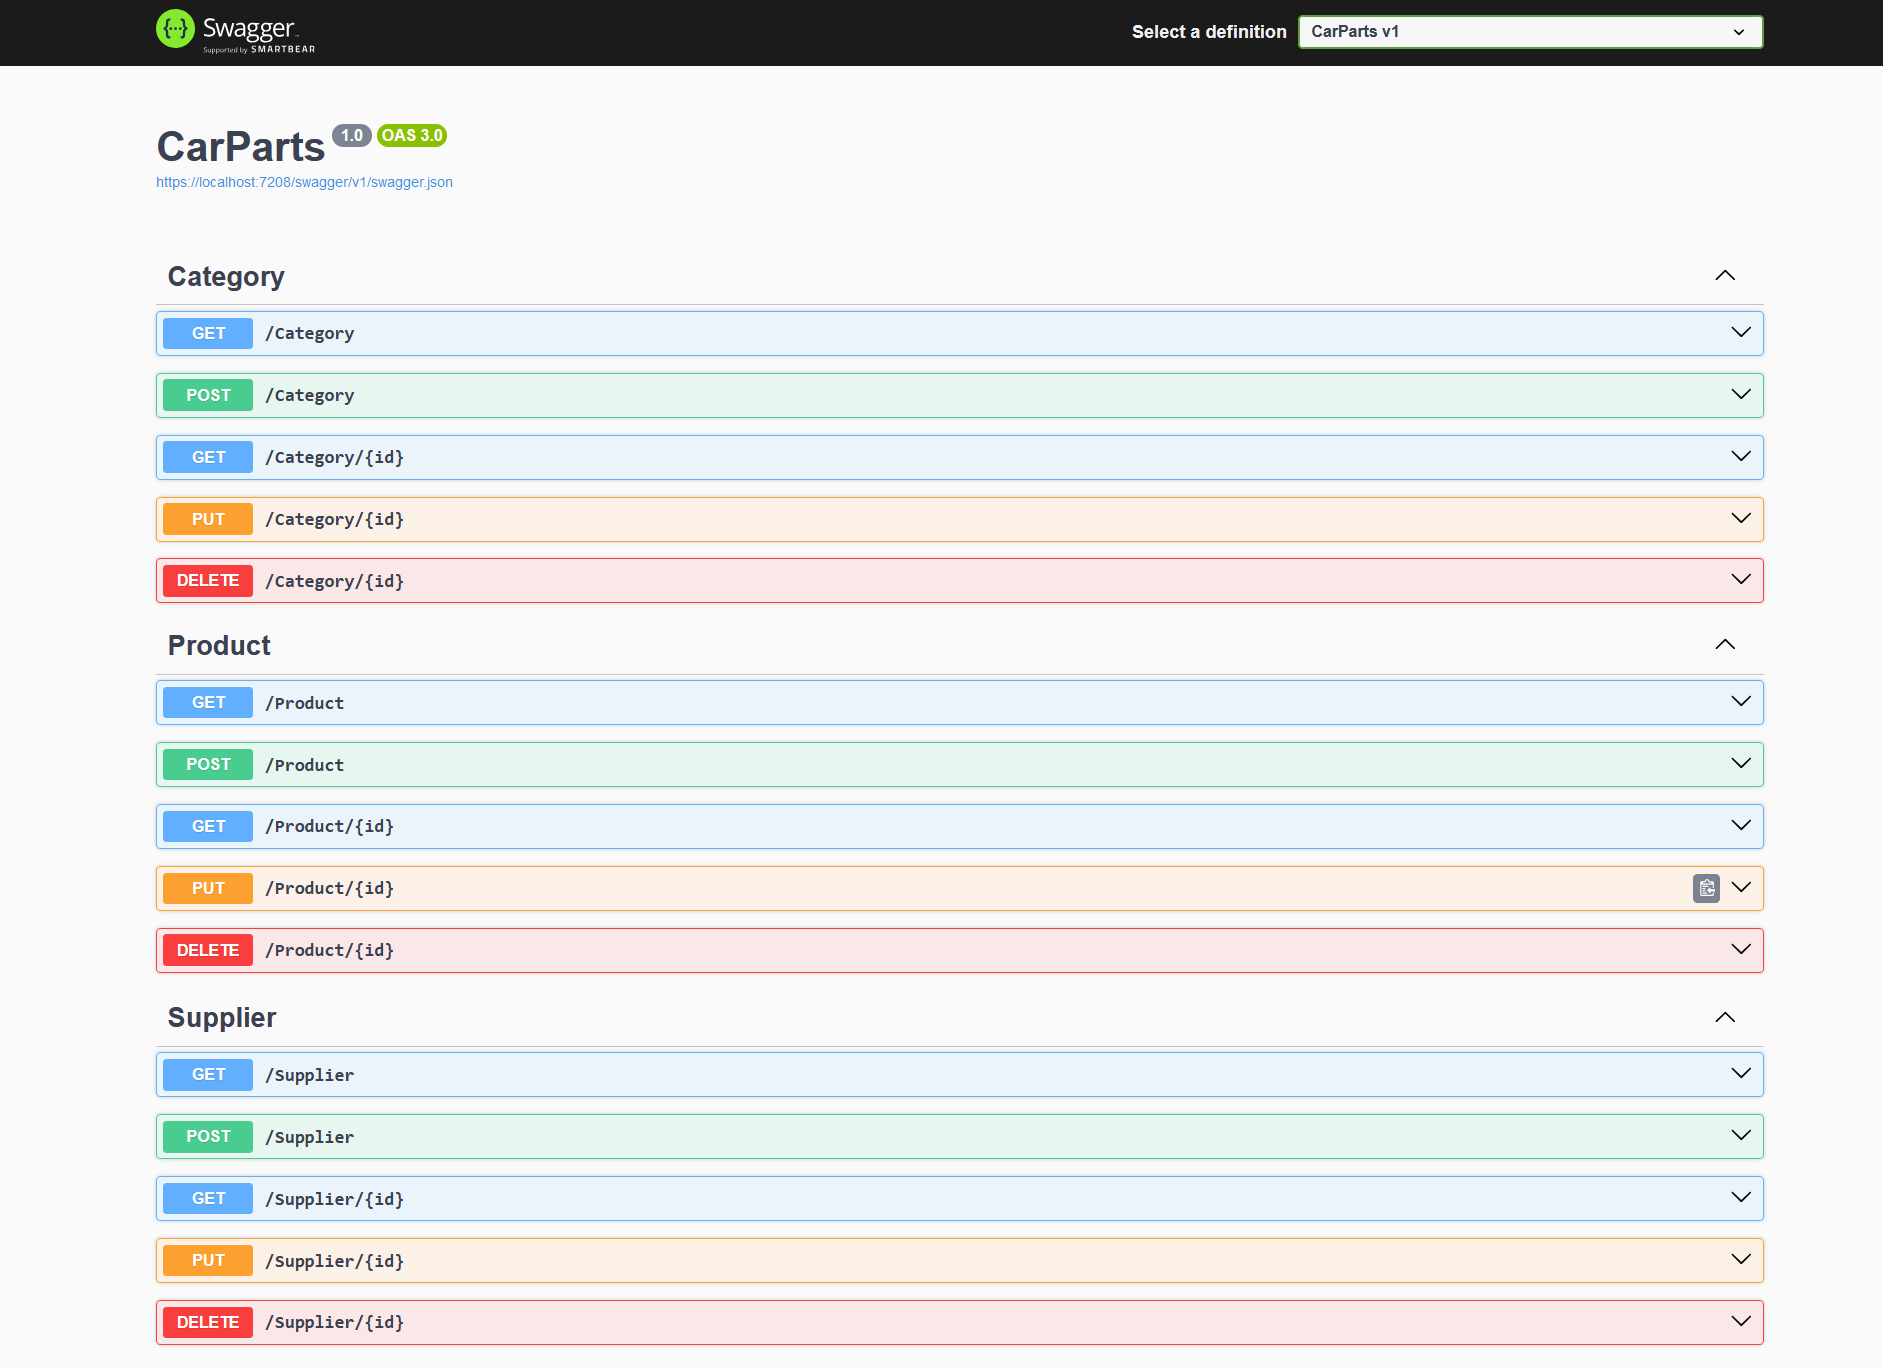
\includegraphics[width=0.8\textwidth]{img_tests/swagger.png}
    \caption{Widok dokumentacji API (Swagger) dla interakcji z backendem aplikacji.}
    \label{fig:swagger}
\end{figure}
% ********** Koniec rozdziału **********